\section{Section 2}

\begin{figure}[H]
    \centering
    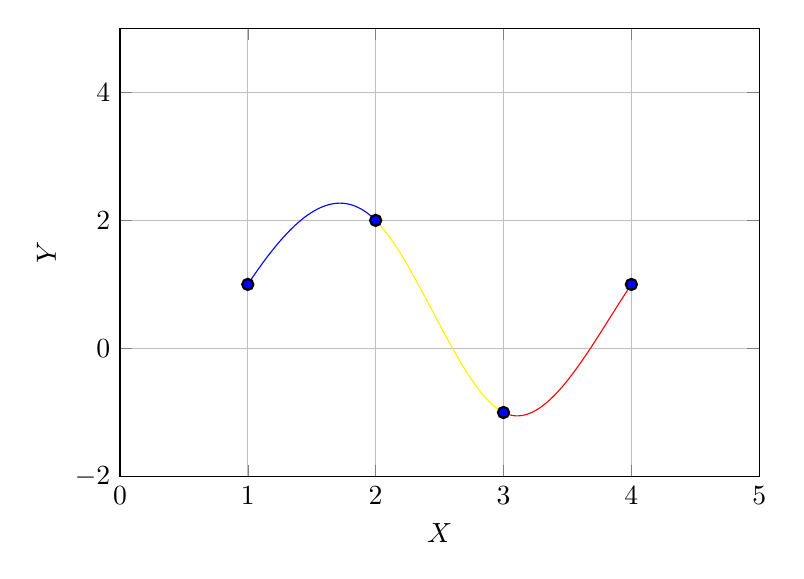
\begin{tikzpicture}
        \begin{axis}
         [
            xlabel = $X$, % Label for X-axis
            ylabel = $Y$, % Label for Y-axis
            grid = both,
            width = 0.8\textwidth,     % Figure width
            height = 0.6\textwidth, % Figure height
            xmin = 0, xmax = 5,  % X-axis limits
            ymin = -2, ymax = 5, % Y-axis limits
         ]
            % Add specific points with custom style
            \addplot[only marks, mark=*, mark options={scale=1, fill=blue, thick}]
            coordinates
            {
                (1,1)
                (2,2)
                (3,-1)
                (4,1)
            };
            % Add piecewise functions (polynomial example)
            \addplot[blue, domain=1:2, samples=500]{1+3*(x-1)-2*(x-1)^2-((x-1)^2)*(x-2)};
            \addplot[yellow, domain=2:3, samples=500]{2-2*(x-2)-(x-2)^2+3*((x-2)^2)*(x-3)};
            \addplot[red, domain=3:4, samples=500]{-1-(x-3)+3*(x-3)^2-2*((x-3)^2)*(x-4)};
        \end{axis}
    \end{tikzpicture}
\end{figure}